\documentclass[11pt,a4paper]{article}
\usepackage[dvipsnames]{xcolor}
\usepackage{amsmath}
\usepackage{amsfonts}
\usepackage{amssymb}
\usepackage{slashed}
\usepackage{graphicx}

\usepackage{pgfgantt}
%\usepackage{graphicx}
\usepackage{rotating}

% geometry
\usepackage[margin=0.5in]{geometry}

% bibliography sorting
\usepackage{natbib}

% math boldface
\usepackage{bm}

% xspace
\usepackage{xspace}

% Line numberring
\usepackage{lineno}

% HyperReferences
\usepackage{hyperref}

% Export Helvetica Fonts
\usepackage[scaled]{helvet}
\renewcommand\familydefault{\sfdefault} 
\usepackage[T1]{fontenc}

%Switch line numbers
%\linenumbers

\newcommand{\fourtop}{\mbox{$t\bar{t}t\bar{t}$}\xspace}
\newcommand{\bbbb}{\mbox{$b\bar{b}b\bar{b}$}\xspace}
\newcommand{\ttbb}{\mbox{$t\bar{t}b\bar{b}$}\xspace}
\newcommand{\hight}{\mbox{$H_T$}\xspace}
\newcommand{\mplank}{\mbox{$\mathrm{M_P}$}\xspace}
\newcommand{\misspt}{\mbox{$\vec{\slashed{p}}_T$}\xspace}
\newcommand{\mycolor}{ForestGreen}

\begin{document}
\begin{center}  
\textbf{\textit{{\Large Indicate the state-of-the-art.}}}\\
\end{center}
\textcolor{\mycolor}{
It is generally accepted that there are four fundamental forces that govern the evolution of the Universe. \textcolor{\mynew}{Three of these (strong, weak and electromagnetic) described in quantum field theory called the Standard Model (SM).} It is believed that the successful resolution of the so called hierarchy problem of particle physics, namely, why the gravitational interaction is many orders of magnitude weaker than other forces, is an essential ingredient to the resolution of a wider problem, the construction of self-consistent description of quantum gravity and a unified theory of all interactions.}

\textcolor{\mycolor}{
The SM describes strong, weak and electromagnetic interactions of elementary matter constituents. Since its inception in the 1960s, the SM was placed under high scrutiny in a vast range of experiments. The predictions of the SM were tested at the scales down to $10^{-19}$m and no significant deviations were observed so far~\cite{Agashe:2014kda}. For example, the perturbative predictions of quantum chromodynamics (QCD), the theory of strong interaction of quarks and gluons, provide a very good agreement in the description of the \textbf{precise measurement of the inclusive-jet cross sections in $ep$ collisions at HERA} (Hadron-Electron Ring Accelerator)~\cite{Abramowicz:2012jz}, to which I made the main contribution.}

\textcolor{\mycolor}{
The discovery in 2012~\cite{Aad:2012tfa,Chatrchyan:2012xdj} of the particle consistent with the Higgs particle, predicted by the BEH (Brout--Englert--Higgs) mechanism of electroweak symmetry breaking, marks a new era of experimental verification of the particle content of the SM. After all, the SM cannot be considered as ultimate theory because it has several limitations. In particular, the SM does not explain a priori why the scale of electroweak symmetry breaking is so much different from the Plank scale, at which all fundamental interactions are supposed to unify. In other words, the SM doesn't answer why gravitational force is much weaker than other interactions. Moreover, the huge difference of about seventeen orders of magnitude between the two scales is considered as very unnatural and suggests to look for mechanisms beyond the SM (BSM), capable to generate such a ``hierarchy'' of scales. In addition, there is neither explanation for observed matter-antimatter asymmetry of the Universe nor for the origin of dark matter and energy.}

\textcolor{\mycolor}{
Various models extending the content of the SM were proposed over the past decades to provide a natural (without excessive fine-tuning of the model parameters) solution to the hierarchy problem. Suggested models can be approximately grouped into several classes including supersymmetric (SUSY) extensions of the SM, models with extra dimensions, composite Higgs and so-called little-Higgs models. \textbf{Most of the proposed solutions predict new particles with enhanced coupling to the heaviest SM particle --- the top quark}\footnote{In what follows, (anti-)top quarks are generically called top and denoted by $t$, unless explicitly stated.}. Among those are models with vector-like quarks~\cite{Aguilar-Saavedra:2013qpa}, models that predict additional massive color-singlet spin-1 $Z'$~\cite{Langacker:2008yv} or composite Higgs~\cite{Agashe:2004rs} boson, models with the so-called Kaluza-Klein (KK) states~\cite{Agashe:2006hk,Davoudiasl:1999jd}, 2HDM model~\cite{Dicus:1994bm,Craig:2015jba,Craig:2016ygr}, as well as those with strongly interacting scalar fields --- sgluons~\cite{Plehn:2008ae,GoncalvesNetto:2012nt}. Although a wealth of theoretically viable models have been proposed, only empirical evidence can establish their verity, therefore the \textbf{search for BSM processes is one of the main objectives of the experiments at the Large Hadron Collider (LHC)}, particularly in the so-called RUN 2 with increased collision energy and therefore larger cross section of hypothetical BSM processes. An observation of such processes will be a \textbf{major breakthrough in the field} after the Higgs boson discovery.}

\textcolor{\mynew}{
Four top quarks production is one promising channel to search for signals of new physics. For example, heavy resonances that couple strongly to top quarks, will result in four tops in the final state, if produced in pairs. Alternatively, if the scale of new physics is too high to be observed directly at the LHC, it can manifest itself as a deviation from the standard model predictions, e.g. an enhancement of $t\bar{t}t\bar{t}$ total cross section due to virtual contribution of BSM states. Being an example of a rare multiparticle process, the SM production of four top quarks is very interesting in its own right, since experimental data can challenge state-of-the art perturbative calculation techniques.
}
\textcolor{\mycolor}{
Two general-purpose experiments at the LHC, ATLAS and CMS, have extensive physics programs dedicated to BSM searches. The state-of-the-art analyses, focused on final states with a top quark signature, utilised $\sqrt{s}=$ 13 TeV data to establish the upper limit on the SM four top quarks production cross section~\cite{Aaboud:2017faq,Sirunyan:2017roi,Sirunyan:2017tep}. These new data can be re-interpreted within the BSM context as, for example, in~\cite{Beck:2015cga}, where %narrow leptophobic $Z'$ and gluon KK resonances decaying to $t\bar{t}$ pairs with a mass below 2.4 and 2.8 TeV, respectively, were excluded at 95\% confidence level (CL) by CMS~\cite{Khachatryan:2015sma}; vector-like charge $2/3e$ T quarks with lower mass limit between 720 and 920 GeV were excluded exploiting events with $ttHH$ and $ttWW$ in the final state~\cite{Khachatryan:2015oba};
the $\sqrt{s}=$ 8 TeV results were used to derive the lower limit on the mass of scalar gluons up to 750 GeV assuming typical sgluon-top coupling values. Alternatively, in~\cite{Cao:2016wib,Sirunyan:2017tep}, limits on four top quarks production were used to obtain the constrains of top-Higgs Yukawa coupling or masses of heavy higgs-like scalars, respectively.}

\textcolor{\mycolor}{
BSM models with enhanced coupling to the top quark are constrained by SUSY searches looking for gluino\footnote{Gluino is a fermionic SUSY partner of the gluon.}-mediated stop\footnote{Stop is a scalar SUSY partner of the top quark.} production~\cite{Sirunyan:2017uyt}. However, in contrast to the study to be pursued in this project, these searches impose very strict requirements on the missing momentum, \misspt, the assumption that undetected weakly interacting particles\footnote{Popular SUSY models, including the MSSM, endowed with the so-called R-symmetry, contain lightest neutral weakly-interacting SUSY particle (LSP) in the mass spectrum. Thus, heavier SUSY partners decay to SM particles and the LSP resulting in significant missing momentum as an experimental signature.} are also produced.}

\textcolor{\mycolor}{
The analyses proposed here exploit properties of the top-quark decays to enrich data samples with hypothetical signal events. Top quarks decay almost exclusively via $t \rightarrow Wb$ channel, therefore initial $t$-selection is typically based on identifying secondary vertices from $b$-decays and leptons or jets from $W$-bosons. Additionally, if the $W$-boson decays via $W\rightarrow l\tilde{\nu}$, a small amount of \misspt is also present in the event and attributed to neutrinos in the SM. }

\textcolor{\mycolor}{
As mentioned, no deviations from predictions of SM were observed so far. Nevertheless, the 2017--2018 $\sqrt{s}=13$ TeV and planned 14 TeV LHC runs have high discovery potential. As demonstrated in~\cite{Sirunyan:2017tep}, the limit on the SM $t\bar{t}t\bar{t}$ can be significantly improved and possibly statistically significant observation of the SM signal can be made, provided the datasets that were accumulated in 2017 and will be collected in 2018. 
Given more than thirty-fold increase of the integrated luminosity of the $\sqrt{s}=13$ dataset in 2016--2017, the LHC may provide a decisive answer to the naturalness problem during the time covered by this proposal. With increased amount of data and potentially $pp$ collision energy, larger mass range and more complex event signatures become accessible at the LHC. To efficiently explore these new signatures, novel analyses strategies will be necessary. Such novel analysis is the subject of this proposal.}

\textcolor{\mycolor}{
Decays of heavy objects, like  aforementioned BSM states, result in large Lorentz-boost of daughter particles, therefore the decay products of the top quark, that originates from such a state, typically overlap in the detector. In order to overcome this problem and achieve high signal selection efficiency and purity\footnote{Efficiency determines the relative amount of signal evens surviving selection procedure, while purity is a measure of background contribution.}, i.e. optimise statistical significance\footnote{For large number of event counts the statistical significance in counting experiments is approximately equal to the ratio $S=N_{\mathrm{sig}}/\sqrt{N_{\mathrm{sig}}+N_{\mathrm{bg}}}$, where $N_{\mathrm{sig}}\left(N_{\mathrm{bg}}\right)$, denotes an estimate of the number of signal (background) events.} of hypothetical signal, dedicated reconstruction procedures are necessary. Above-mentioned studies utilised multivariate analysis (MVA) methods and I propose to also use jet-substructure techniques to tackle this problem. Currently, development and optimisation of reconstruction and identification algorithms for boosted objects is an extremely active area of research in both experimental and theoretical communities.}

\textcolor{\mycolor}{
The investigation of processes with multi-top-quark signature will be an important milestone in coming years and one of the main paths to indirect observation of new physics at the energy frontier. Such a discovery would likely be the start of a new revolution in fundamental physics. }


\begin{center}
\textbf{\textit{{\Large Describe the objectives of the research.}}}\\
\end{center}
\begin{figure}
\centering
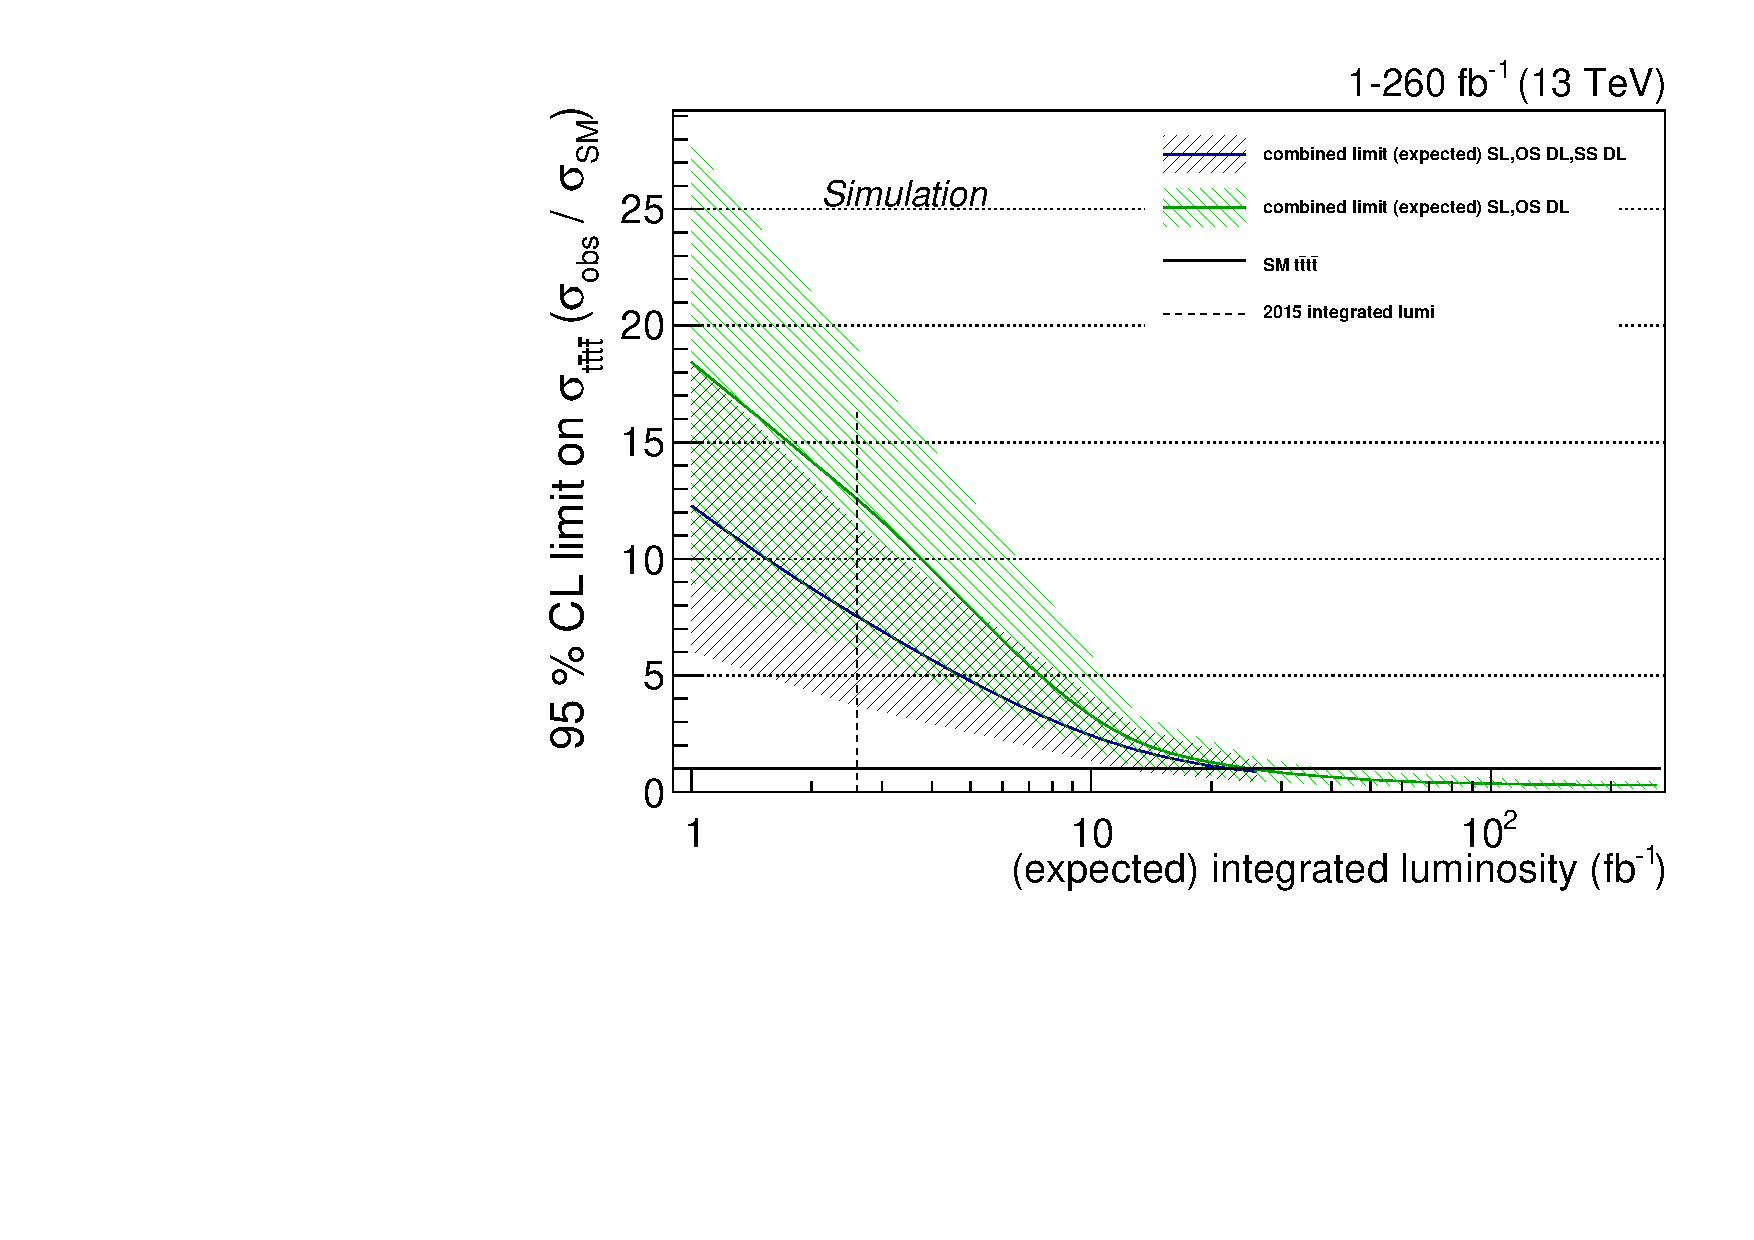
\includegraphics[width=0.45\linewidth]{./figures/combined_limitvslumi_fwo}
\caption{Extrapolation, based on 2015 results~\cite{CMS:2016wig}, of the expected limit on the SM four top quark production cross section as a function of integrated luminosity of the dataset. Solid lines and hatched areas show expected limit dependence and one standard deviation uncertainty band, respectively, for single-lepton (SL) and opposite-sign di-lepton (OS DL) SM $t\bar{t}t\bar{t}$ search (blue) and single-lepton and same (SS DL) and opposite-sign dilepton search (green). The predictions performed assuming that the experimental uncertainty is dominated by statistical component. Even in the case of downward statistical fluctuation, the dataset  delivered during the time covered by this proposal (120 fb$^{-1}$) will be sufficient to observe this process.}
\label{fig:combined_limitvslumi}
\end{figure}
With this project \textbf{I plan to perform direct search for BSM processes in events with $\pmb{t\bar{t}t\bar{t}}$ signature  as well as measure four top quark production in $pp$ collisions with the CMS detector at the LHC at centre-of-mass energy $\sqrt{s}=$ 13 and 14 TeV.} The SM measurement aims at testing the state-of-the-art perturbative QCD predictions~\cite{Bevilacqua:2012em} while direct searches seek for BSM signal. As described above, there is a certain class of models predicting significantly larger than SM cross section values and resonances~\cite{Lillie:2007hd, Gregoire:2011ka, Pomarol:2008bh}, thus making direct test of such models at the LHC feasible in the RUN2 for which, in total, more than 100 fb$^{-1}$ of the integrated luminosity are expected. The discovery of significant deviation from the SM predictions may have a major impact on the field, while the converse will help to restrict possible BSM scenarios. The recent constraints from $\sqrt{s}=13$ TeV data for SM four top production at ATLAS~\cite{ATLAS:2016gqb} and CMS~\cite{CMS:2016wig,Beck:2016hyi}, to which I have made a significant contribution,
%~\cite{Aad:2015kqa,Khachatryan:2014sca} 
resulted in 193 (147) and 93 (99) fb observed (expected) 95\% CL upper limits on the production cross section, respectively, that is more than 10 times larger than the SM predictions, therefore new physics models could be hidden until the analyses have greater sensitivity with larger dataset.

The previous analysis at CMS made use of 2.3 fb$^{-1}$ of integrated luminosity, that is about 20 signal events for the complete 2015 dataset. \textbf{I plan to analyse full data sample collected in 2016--2017 to increase statistical and systematic precision of the search} which will significantly increase the sensitivity to the processes with four top quarks. 

Examples of leading order (LO) SM and corresponding BSM Feynman diagrams for $t\bar{t}t\bar{t}$ production are illustrated in Figure~\ref{fig:LOtttt}. The reconstruction of this process is especially challenging because such final state is characterised by large hadronic activity, $\hight$, and incorporates four b-quarks, jets or leptons from $W$-decays and additional jets from initial and/or final-state QCD radiation. In addition, such events have non-vanishing missing momentum in case of semileptonic $W$-decays, which is reasonably well under control in top physics. Beauty quarks are identified exploiting the properties of the weak decays of $B$-hadrons, which are typically formed from $b$'s during the hadronisation stage. These hadrons have relatively long mean lifetime of the order of 10$^{-12}$s and travel several millimeters from the production point before they decay giving rise to displaced tracks. Depending on the decay channel of $W$-bosons, several possible combinations of jet and lepton multiplicities can be identified in \fourtop events e.g. final states with a single muon $\left(\mu\right)$+jets or a single electron $\left(e\right)$+jets\footnote{In the following, charged first and second generation leptons, i.e. $e/\mu$ are generically denoted by $l$.} arising promptly from $W$ decays or in a cascade $W\rightarrow\tau\nu_\tau$, $\tau\rightarrow l\nu_l \nu_\tau$. This final state has the highest probability ($\approx 41\%$) of occurrence, while zero-leptons, two-leptons or three- and four-leptons have 30\%, 22\% and 6\% odds, respectively~\cite{Khachatryan:2014sca}.  Vanishing $\misspt$ in the all-hadronic channel as well as the capability to reconstruct the momentum of the neutrino\footnote{The SM decay hypothesis of the $W$ boson has to be assumed} in the single-lepton channel, increases the sensitivity to BSM models without undetectable particles carrying significant momentum. This signature makes this proposal \textbf{unique as no similar analyses, besides ongoing effort of the applicant and the hosting group, are currently being performed by the CMS collaboration}.

\begin{figure}[t!]
\centering
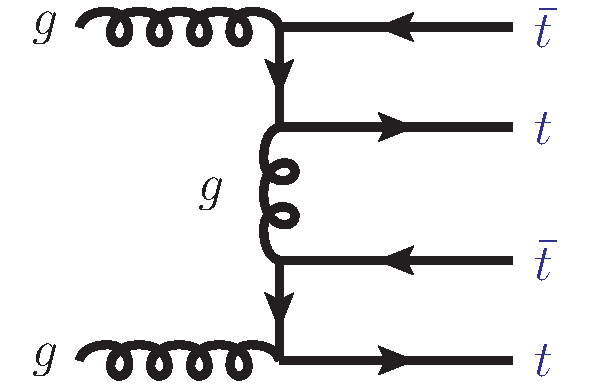
\includegraphics[width=0.25\textwidth]{Feynman/gg2tttt}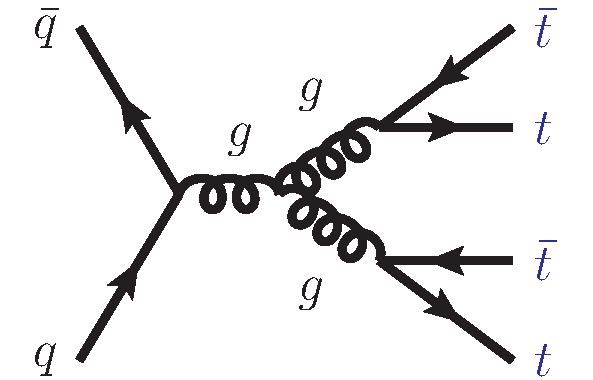
\includegraphics[width=0.25\textwidth]{Feynman/qq2tttt}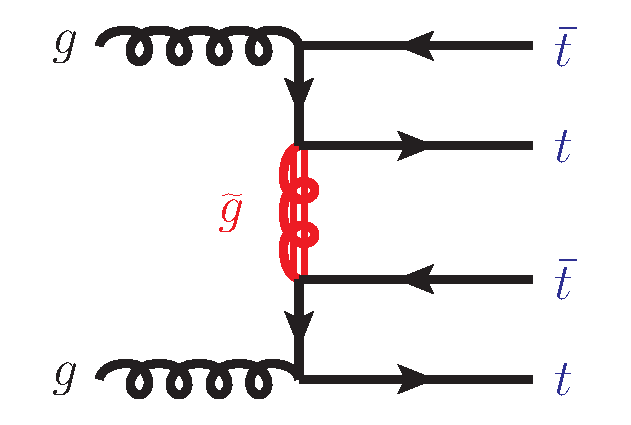
\includegraphics[width=0.25\textwidth]{Feynman/gg2ttttsgluon}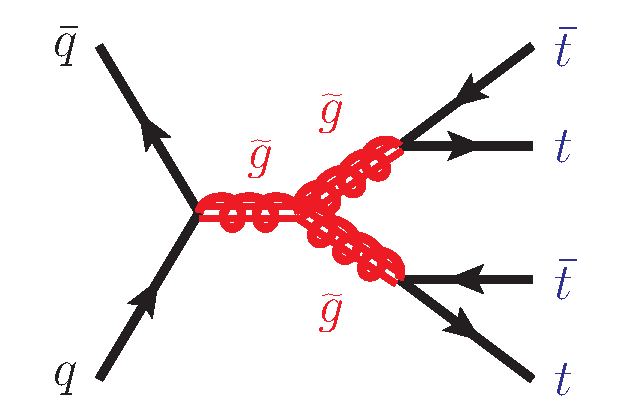
\includegraphics[width=0.25\textwidth]{Feynman/qq2ttttsgluon}
\caption{Examples of leading order SM and corresponding BSM Feynman diagrams for $t\bar{t}t\bar{t}$ production. The intermediate states, indicated by $\tilde{g}$, represent coloured scalar fields -- sgluons.}
\label{fig:LOtttt}
\end{figure}

Several principal challenges inherent to the explored final state can be identified early on. 
%An efficient $b$-tagging algorithm with high discriminating power at high jet multiplicity is crucial for selection of four top events and suppression of overwhelming background, mostly comprised of $t\bar{t}jj$ production, where $jj$ denotes a pair of light-flavour\footnote{Jets originating from $u,d,s,g$ partons are generically called light-flavour jets.} or $c$-quark jets, or associated electroweak-boson production. The CMS collaboration relies on well established algorithms~\cite{Chatrchyan:2012jua} for this task. However, their settings were optimised for the physics environment of $\sqrt{s}=7(8)$ TeV runs~\cite{CMS:2013vea}, whereas due to increased energy and pile-up in RUN2, their performance may not be optimal anymore. Besides the pile-up effect, $b$-tagging may also be affected by the complex multijet signature of the proposed signal. Thus, \textbf{investigation and optimisation of $b$-tagging performance} in the complex $t\bar{t}t\bar{t}$ environment at $\sqrt{s}=$ 13(14) TeV is envisaged in this project. These results can be later used in other analyses with similar event signatures. 
A difficulty persistent to the reconstruction of multiple top quarks is identification of a correct combination of final state objects arising from a common mother-particle decay. For example, in the single-lepton channel, $4!\cdot C_6^2 \cdot C_4^2 = 2160$, where $C_n^k$ denotes binomial coefficient, possible assignments of four $b$-jets and six light-flavour jets to four top quarks exist. In order to suppress combinatorial background, decay products kinematic information can be used, e.g. combinations with invariant masses outside $W$-boson and top-quark mass windows can be rejected. Furthermore, MVA techniques can be applied to enhance classification power of assignment algorithm. The \textbf{improvement in the top-decay reconstruction} will have a significant impact on the signal sensitivity and background suppression.

The details of the suggested solutions to foreseen challenges as well as the generic strategy for reaching the objectives of this proposal are outlined below.
%The principal goal and major challenges can be 
% 
%\textbf{TODO:}\\
%- Describe how to search for four top events. Many jets, many b's,\\
%\hfill
%+ Test of the SM predictions and search for BSM signatures.\\
%+ So far 32fb-1 limit was established while SM cross section is only 1fb-1 and this gives a huge room where to hide for new physics.\\
%+ It is very important and will have a huge impact in case of discovery and will place strict limits on possible BSM scenarios.\\
%+ It is very challenging because of overwhelming SM background, possibly not enough efficient b-tagging etc.;
%+++ enumerate probabilities for four top decay channels+++
%+++Mention b-classification efficiency+++ 
%+++Mention combinatorics problem+++ 
%+++Mention QCD background+++ 
%+++Mention non-optimal b-tagging for increased pile-up/boosted jets (timely)+++
%+++Mention possibly non-optimal trigger+++

\begin{center}
\textbf{\textit{{\Large Describe the methodology of your research.}}}\\
\end{center}
\textcolor{\mycolor}{
From experimental point of view, the process cross section can be determined applying generic formula:
\begin{equation}
\sigma = \left(N_{\mathrm{sig}}-N_{\mathrm{bg}}\right)\cdot \mathcal{A} \cdot \mathcal{L}^{-1},
\label{eq:csdef}
\end{equation}
where $N_{\mathrm{sig}}\left(N_{\mathrm{bg}}\right)$, denotes an estimate of the number of signal (background) events, while $\mathcal{L}$ and $\mathcal{A}$ represent an integrated luminosity and a correction factor taking detector and possibly other effects into account, respectively. }

\textcolor{\mycolor}{
As follows from the Eq.~\eqref{eq:csdef}, to measure the process cross section, typically several steps have to be performed, i.e. the number of signal and background events as well as the integrated luminosity have to be determined for a given data sample; the detector effects attributed to e.g. inefficiencies, finite resolution, etc. also have to be taken into account. On the other hand, in the direct searchers for new phenomena, typically the regions of phase space are investigated in which the signal production cross section is enhanced and exceeds the background significantly. In general, in this procedure certain assumptions about e.g. modelling of the detector response or the shape of the background spectrum are typically made. The sensitivity of the result to variations of different assumptions is called systematic uncertainty and is one of the crucial components of the analysis that often requires elaborate studies. Besides that, the precision of the measurements with low event count rate as e.g. \fourtop production, is usually limited by stochastic effects\footnote{Typically attributed to statistical uncertainty on the number of signal events.}, which also have to be properly taken into account. To achieve all mentioned tasks, various techniques, employing simulations of relevant processes, data-driven analysis methods and statistical means, exist. The proposed research follows closely well established paradigm in the field. The foreseen steps and intermediate goals of this study are detailed below.}

\textcolor{\mycolor}{
Depending on the principal task, i.e. measurement of the SM cross section or direct search for BSM signal, two corresponding sub-projects can be identified in this proposal. In general, any experimental analysis aims at best measurement precision, however, in case of searches for new phenomena, the maximal statistical significance of the signal is required in addition.
% The $b$- and $t$-reconstruction and tagging algorithms, to be described below, are being developed in order to minimise background contamination, $N_{\mathrm{bg}}$, and to reconstruct maximum possible number of signal events, $N_{\mathrm{sig}}$ in case of direct searches, and to be maximally robust against detector effects in case of cross section measurement. As follows from Eq.~\ref{eq:csdef}, 
%
Two different strategies will be pursued in the respective sub-projects, however both can be performed using comparable tools. Furthermore, it is natural to split the sub-projects further according to the $t\bar{t}t\bar{t}$ decay channel to be considered, corresponding to zero-, single- and two-lepton final states, respectively. As all three have different experimental signatures, development and optimisation of individual reconstruction algorithms, selection of appropriate trigger chains, background studies as well as determination of statistical and systematic effects will be different in three sub-projects. However, they have a common core related to the reconstruction and identification of $b$-quark jets and reconstruction of hadronic top decays.}

\textcolor{\mycolor}{The single-lepton channel, previously studied in~\cite{CMS:2016wig,Beck:2016hyi} and~\cite{Khachatryan:2014sca} is considered the most straight-forward analysis in this project. It has the largest branching fraction and expected to have moderate background level. Moreover, constrained-kinematics reconstruction, extensively employed in CMS in top-pair production analyses, is directly applicable in this channel and will have significant effect on top quark identification efficiency. This sub-project will largely benefit from extensive experience of the host institution in this analysis and will use state-of-the-art dedicated tools developed there.} \begin{figure}
\centering
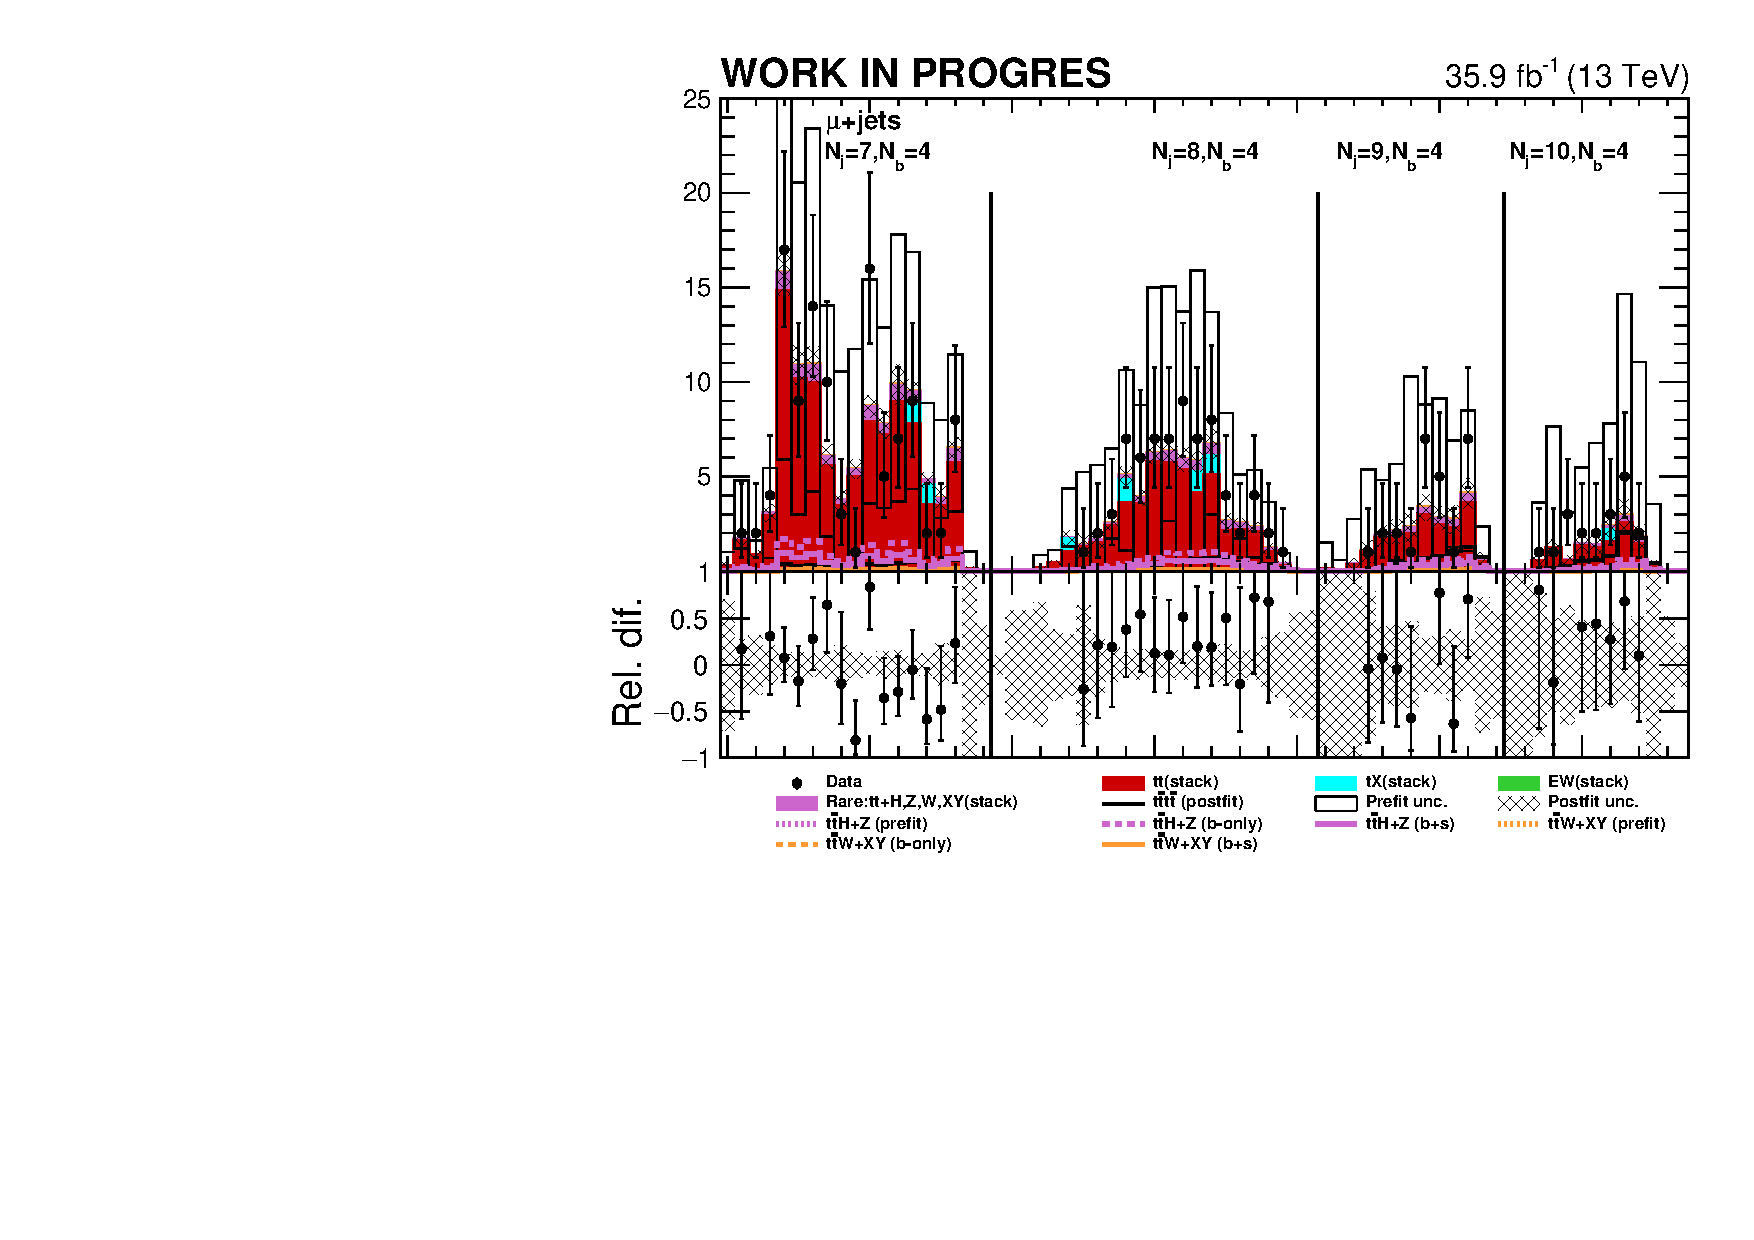
\includegraphics[width=\linewidth]{figures/mu}
\caption{\textbf{Work in progress.} Distribution of MVA discriminant in the most sensitive search regions in $\mu+$jets channel obtained using 35.9 \invfb dataset collected during 2016 data tacking period. Observations are shown as black dots, while background predictions obtained from Monte Carlo simulations are shown as a stacked histogram. A prioty uncertainty on the MC predictions are shown as open squares and uncertainties obtained from the fit to the data in control regions are shown as hatched area. Bottom panel of the figure demonstrates relative difference of the data with respect to background predictions.}
\label{fig:mu}
\end{figure}
Analysis framework for event selection and resolved hadronic top decays reconstruction is already developed and interfaced with statistical interpretation software. Preliminary results have been obtained using 35.9 \invfb of integrated luminosity collected in 2016. Fig.~\ref{fig:mu} shows multivariate discriminant distributions in the most sensitive search regions. An \textbf{excess} of signal over SM predictions was observed, but further studies are necessary to understand the nature of the signal. The results obtained in same-sign dilepton and multilepton channels~\cite{Sirunyan:2017roi} do not confirm this \textbf{preliminary} observation, therefore further research in single-lepton channel is required to claim an observation. \textbf{It will be crucial to continue analysing 2016--2017 data in this channel to confirm or rule out the excess.} In general, the direct search in this channel represents the minimal goal of the proposal. The results of this study using 2016--2017 data are already novel enough to be published in a peer-reviewed journal. 

To complete the analysis and draw the conclusions about the impact of new searches, the data can be interpreted within the so-called effective-field theory (EFT) approach~\cite{Lillie:2007hd} in which the impact of BSM physics is parametrised by higher-dimensional operators constructed from the products of SM fields. In my opinion, this is the optimal approach, because these results, in contrast to a particular ultraviolet-complete model, can, at least in principle, be reinterpreted within any given BSM model. The EFT-analysis of the measurements is a novel approach to the interpretation of the $t\bar{t}t\bar{t}$ data and may attract larger attention to the obtained results. The outcome of this analysis can be presented as a \textbf{separate publication} or together with the results of the searches. 

A work on EFT interpretation has been carried out in parallel to the 2016 data analysis. Fig.~\ref{fig:C1_C2} demonstrates the marginalised constrains on dimension-6 four-fermion operators contributing to four top quarks production at the LHC~\cite{DegrandeEFTthesis,Zhang:2017mls}. As can be seen, significant improvement can be achieved with larger Run 2 datasample.
\begin{figure}[h]
\centering
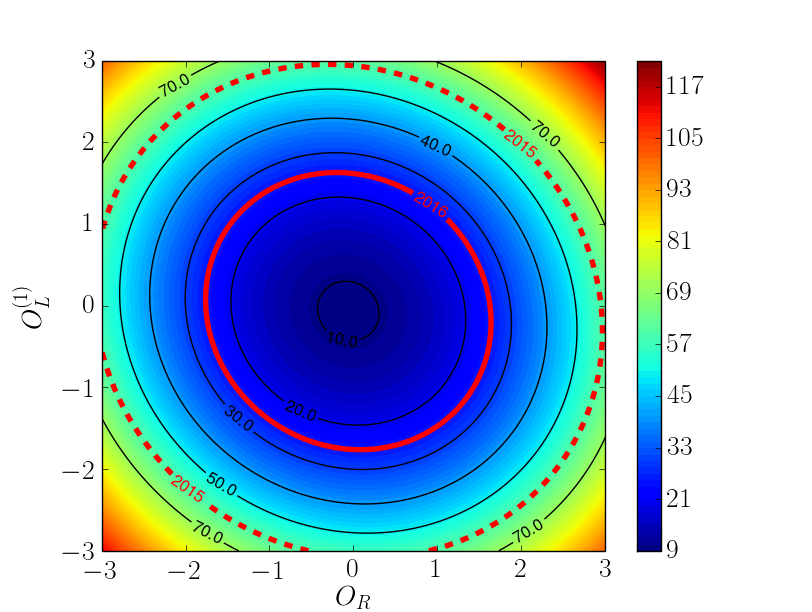
\includegraphics[width=0.7\linewidth]{figures/C1_C2}
\caption{\textbf{Work in progress.} Independent limits on four fermion dimension 6 operators $O_{L}^{\left(1 \right) }$ and $O_R$, defined in~\cite{DegrandeEFTthesis}, that can be obtained using 2015 (dashed line) or 2016 (solid line) datasets. The region outside red dashed or solid ellipses are excluded by observations. Color axis represents predictions for four top total cross section, $\sigma_{t\bar{t}t\bar{t}}$, for given values of effective coupling parameters (Wilson coefficients) of $O_{L}^{\left(1 \right) }$ and $O_R$ operators.}
\label{fig:C1_C2}
\end{figure} 

Determination of the $t\bar{t}t\bar{t}$ production cross section in other channels and corresponding searches are a logical extension of the described analysis. The two-lepton channel can provide a valuable contribution with a moderate effort, while the analysis in the zero-lepton channel may present significant challenge due to major difference in the final-state. In this case \textbf{my experience in jet analyses will be especially suitable for developing dedicated tools for hadronic top decay} reconstruction.

In order to reach the ultimate sensitivity in the BSM searches, the next logical step, contingent with these sub-tasks, is a combination and interpretation of the results obtained in various channels. They will perfectly fit together with the analysis of the single-lepton channel, but can be issued together with the combination in a \textbf{separate publication}.

To fulfill the ambitious plans outlined above, the research will be delivered in three work-packages which are elucidated in the following.
% baseline selection and event reconstruction
% interpretation of the results within specific and EFT models. Cite Chen:2014ewl

\begin{center}
\textbf{\textit{{\Large Provide a work plan, i.e. the different work packages (WPs) and a detailed timetable.}}}\\
\end{center}
% investigation and optimisation of 
%	possible trigger optimisation
%	b-tagging (pile-up, boost/sub-jets, new layer(timely)), jet-charge, PUPPI
%	top-tagging (sub-jets, kinematic reconstruction, MVA/Matrix-Element etc.)
% measurement of cross section and evaluation of systematic uncertainties
%timetable
\noindent\textit{1. Trigger-chain selection and optimisation; $t\bar{t}t\bar{t}$ process baseline selection. (low-risk)}\\
To select candidate \fourtop events on-line, different existing CMS trigger paths will be used depending on the decay channel in focus. Thus, for example, dedicated single-muon and single-electron triggers can be utilised for $l$+jets channel, while the $ll$+jets selection can take the advantage of existing di-lepton triggers. Presence of a $b$-jet can be possibly included to the High-Level trigger requirements also. For the all-hadronic \fourtop channel no dedicated triggers exist, however, the applicability of CMS multi-jet and high-$\hight$ trigger chains developed for SUSY analyses can be explored, otherwise a\textbf{ dedicated trigger path will be designed} for the 2017--2018 running phase. In case such a trigger configuration will be developed, one can benefit from tunning the trigger specifically to have high acceptance for \fourtop events, for example $p_T$ thresholds can be lowered while maintaining acceptable trigger rates. Well established techniques will be used to measure efficiencies and corresponding systematic uncertainties attributed to those triggers. I have \textbf{experience in both development and optimising new trigger} configuration as well as the measurements of existing trigger performance. Therefore this task is considered as having a \textbf{low risk} and is a natural starting point for further deployment of the analysis.
\newline
%
%\noindent\textit{2. $b$-tagging performance optimisation. (medium-risk)}\\
%After selecting suitable trigger chains and ensuring appropriate quality of selected final-state leptons and jets using off-line selection criteria, further restrictions on $b$- and light-flavour-jet multiplicity will be imposed to reduce the background from top-pair production associated with multiple jets. Any particular choice is always a trade-off between selection efficiency and purity of the data sample, and thus is subject to optimisation.

After imposing appropriate selection criteria on $b$-quark multiplicity, the remaining dominant background contribution will be due to \ttbb, for zero-leptons or single- and two-leptons channels, respectively. The production cross sections of \ttbb process is approximately two orders of magnitude larger~\cite{Bevilacqua:2014qfa} than that of \fourtop. For this reason, the next logical step would be to identify and reconstruct (additional) top decays.
%\newline

\noindent\textit{2. The SM $t\bar{t}t\bar{t}$ production measurement. (low-risk)}\\
In case no deviations from the SM will be found and given that the systematic and statistical uncertainties analysis framework will be established, in principle, the direct searches can be turned into the measurement of the SM \fourtop production cross section with a reasonable effort. In this case, in contrast to the direct searches, probably a wider phase space can be investigated in order to increase the amount of the SM signal \fourtop events. Thus, additional studies of the description of the data by the simulations might be needed in order to ensure reliability of the estimates of the detector effects in a wider phase space. 

\textbf{This analysis is a natural extension of the results obtained using 2015 dataset~\cite{CMS:2016wig}. My experience here makes me an ideal candidate to carry out this project that can be used as a back-up scenario ``if everything else fails''.} As demonstrated in Fig.~\ref{fig:combined_limitvslumi}, even in case of downward statistical fluctuation, the future dataset collected in 2017--2018 will be sufficient to make an observation. Therefore this WP is considered as low-risk.

The Standard Model measurement in of the \fourtop production cross sections in different channels will be \textbf{published in a refereed journal}.
\newline


\noindent\textit{3. Top-tagging performance optimisation. (medium-risk)}\\
\textcolor{\mynew}{
The standard model four top production is characterised by moderate transverse momentum of produced tops, therefore decay products can be resolved in the detector. At $\sqrt{s}$=14 TeV, however, a significant fraction of top quarks is expected to be produced with large Lorentz-boost, leading to strongly collimated decay products which end-up in a single jet. 
Moreover, as was mentioned, many BSM models predict heavy states, resulting in a large boost of the decay products. Thus the searches for such states in resolved topology events, as in WP1, are less efficient and reconstruction of boosted top decays becomes crucial for direct searches. 
}
\textcolor{\mynew}{
The top-tagging is currently an active area of research and many novel techniques were proposed over the last years. In particular, the HepTopTagger algorithm~\cite{heptoptagger} demonstrated very good performance in the recent search for pair production of vector-like T quarks in events with similar event signature in CMS~\cite{Khachatryan:2015oba}. Besides that, the CMSTopTagger~\cite{Kaplan:2008ie} employs a different jet deconstruction approach which is more suitable for highly boosted top decays. More algorithms exist including shower-deconstruction tagger and N-subjettiness algorithm, the applicability of which~\cite{CMS:2014fya} still has to be explored. Therefore, in order to enhance sensitivity to BSM \fourtop signal, especially in the zero-leptons decay channel, the investigation of different techniques is foreseen in this project. To my knowledge, besides the discontinued attempt of $W$-tagging at UGent, this can be the \textbf{first significant effort on jet substructure in Belgium}.
}
\textcolor{\mynew}{
This task goes hand-in-hand with optimisation of the $b$-tagging in sub-jet environment. A better performance of the $b$-tagging can give a significant gain in terms of light-flavour background rejection, therefore I plan to investigate novel tools designed in CMS~\cite{Bertolini:2014bba} and explore new promising jet-charge identification technique developed recently in ATLAS~\cite{Aad:2015cua,ATLAS:2015jetcharge}.
}
\textcolor{\mynew}{
This WP is exploratory in nature and assessed as a \textbf{high-risk and high-impact}. This effort is very timely with the LHC instantaneous luminosity increase foreseen for the year 2018 and may have a positive impact for other studies in the collaboration, for example, for 'high-profile' $ttH \rightarrow ttb\bar{b}$ search planned to be performed by the hosting group. The all-hadronic channel may require more significant effort investment. There are diverse challenges inherent to severe not completely understood QCD background. In addition, input from CMS collaborators on performance of b-tagging algorithms in boosted regime is needed. Eventually, the success in this project relies on novel tools. Nevertheless, I believe, I am a perfect candidate for this pioneering effort, since I have a wide knowledge acquired during my doctoral studies in the area of track reconstruction and broad experience in jet and top analyses.
}
\textcolor{\mynew}{
Without doubt, the discovery of a new state will have major impact on the field, but negative result is also worth an effort since very little is known about this extreme corner of phase space. The obtained results will be \textbf{published in a refereed journal}. As previously mentioned, the development of substructure algorithms is of great interest in the field. Therefore, it is expected that new developments will be included in a \textbf{performance paper} by the CMS collaboration.
}
%A more general approach to top tagging, applicable in both boosted and un-boosted topologies, is the Matrix-Element (ME) method. In the ME method, a statistical classifier based on final-state kinematic information and LO matrix elements is constructed to test how likely is that given event originates from signal or background source. This technique was recently demonstrated in $ttH \rightarrow ttbb$ analysis~\cite{MartixElementMethod} and proved to be very effective. In addition to that, the approach can be generalised to decide, for example, whether a given combination of jets and leptons arise from the common top decay. Nevertheless, using theoretical input in the selection procedure, unavoidably introduces model dependence in the measurements. Therefore I propose a possibly novel approach in which this problem can be facilitated by combining ME method with MVA techniques. I propose instead of using weights (which are typically available at LO only) directly in the statistical classifier, to utilise them for seeding multivariate regression model to derive improved weights using available higher-order calculations and/or data.

%The studies for single- and two-leptons channels will largely benefit from the experience developed by the host institute, while in the zero-leptons channel my expertise in QCD jet analysis will be a valuable complement.%As described above, the reconstruction of \fourtop final-state suffers from combinatorial ambiguity in assigning the decay products to theirs parent $t$-quarks. This feature helps to mitigate combinatorial problem, because it suggests natural candidates for decay products originating from the same parton. 

%In the single-lepton channel one can benefit from the constrained kinematics of the event. If the lepton is well isolated and its momentum is reliably measured, the four-momentum of the neutrino from the $W$ decay can be reconstructed as well. Considering a single $t\bar{t}$ pair, four equations: momentum conservation, two constraints due to the $W^\pm$ mass and equality of $t$ and $\bar{t}$ masses, can be used to determine four unknown components of the neutrino momentum vector. This information will help to improve the resolution of the various quantities derived from the momenta of final-state objects. In principle, same technique can be applied in the zero-lepton channel as well, although due to much worse precision of the jet measurement and even larger combinatorial ambiguity, the solution of the constrain equations can be less robust.
\newline


\noindent\textit{4. Direct searches for beyond Standard Model processes. (high-risk)}\\
Whenever the data sample is fixed, the search for new signal is a well-established process. A fit to the multivariate discriminator distribution will be performed in order to estimate the amount of \fourtop events in selected samples. In this analysis a significant fraction of the background contamination is expected in the final datasets, therefore its shape and normalisation have to be determined preferably using data-driven approaches or employing theoretical predictions. A simultaneous fit to different background- (signal-) enhanced event categories can be performed to constrain the background and determine the number of signal events. I have a good knowledge of various fitting approaches, including multidimensional likelihood fits to the distributions with low counting statistics to effectively work on this task.

In both BSM searches and SM measurement (see below) the experimental and theoretical sources of systematic uncertainty have to be taken into account as both can affect the shape and normalisation of the measured distributions. Examples of theoretical uncertainty include the ones due to the variation of renormalisation and factorisation scales in perturbative calculations or the variation of the matching scale in the parton-shower-matching procedure. The experimental uncertainties arise, for example, due to finite jet and lepton energy resolutions, b- and top-identification procedures, luminosity etc. These uncertainties can be included as a nuisance parameters into the above-mentioned likelihood fits.

Individual channels will differ in the details of systematic studies, mainly because of the variations in the background strength and sources composition. The studies for single- and two-leptons channels will largely benefit from the experience developed by the host institute, while in the zero-leptons channel my expertise in QCD jet analysis will be a valuable complement.

\textbf{Overall, the described work package is assessed as high risk because it is contingent upon the progress in the previous WP. Moreover, the all-hadronic channel may require more significant effort investment, because of severe QCD background that is not completely understood}. Without doubt, the discovery of a new state will have major impact on the field, but negative result is also worth an effort since very little is known about this extreme corner of phase space. The obtained results will be \textbf{published in a refereed journal}.
\newline

%4.1 $l$+jets channel. (low-risk)
%4.2 $ll$+jets channel. (medium-risk)
%4.3 all jets channel. (high-risk)

\textit{5. Results combination and interpretation. (low/medium-risk)}\\
\textcolor{\mynew}{
The aim of this WP is to perform statistical combination the results obtained in different channels and interpret searches performed in WP1 and WP2 using phenomenological models. As was shown by the applicant in~\cite{Sirunyan:2017tep}, combination of SM \tttt searches in different channels can substantially improve the sensitivity of the search, due to complementarity of information provided by different channels. Although, the improvement in the referenced publication, is attributed mainly to increase of the signal efficiency due to summing contributions from different decay modes, the synergy of independent channels will become more prominent, when statistical component of the uncertainty can be reduced using larger datasets accumulated in 2016--2018. For example, rates of rare backgrounds, such as $t\bar{t}Z$ and $t\bar{t}W$, contributing in both single-lepton and dilepton channels can be better constrained in dedicated control regions of dilepton analysis and applied in single-lepton search. On the other hand, dilepton analysis can profit from larger branching fraction of $t\bar{t} \rightarrow l+\mathrm{jets}$ to better constrain jet multiplicity spectrum, the modelling of which was among dominant sources systematic uncertainty, so far. Combination will be performed using statistics tools, that are widely used in ATLAS and CMS experiments. The applicant has all necessary skills to effectively accomplish this task.
}
\textcolor{\mynew}{
A novel goal of this WP is a bottom-up interpretation of the results of the searches using four top EFT model~\cite{DegrandeEFTthesis}. In case, when no BSM states will be observed, the limits on coupling of effective operators will provide constraints on potential physics scenario beyond the standard model. In contrast to phenomenological interpretation using specific BSM models, such as e.g.~\cite{Sirunyan:2017uyt}, where very restrictive assumptions on model parameters had to be made ($\tan \beta=$1\footnote{In this analysis, the so-called 2HDM model was considered, where $\tan \beta$ is a ratio of vacuum expectation values of $H_u$ and $H_v$ fields.}), EFT analysis helps to draw more universal conclusions about potential new physics. Thus, such results will extend the scope and impact of existing interpretations of four top production data. 
}
\textcolor{\mynew}{
An initial attempt of EFT interpretation of 2015 results, described above, \textbf{demonstrates the potential of new data and my capability to successfully perform this sub-project}. The outlined analysis, is limited by assumption that detector acceptance of \tttt final state resulting from effective interaction of top quarks is the same as for SM \tttt production, which is not the case if the EFT cut-off scale is high, as mentioned in WP2. In order avoid potential ambiguities, the impact on experimental sensitivity of  differences in two production mechanisms will be taken into account in detailed CMS simulations of EFT processes. There are only 5 dim-6 four-fermion operators contributing to production of four top quarks in proton-proton collisions. However, model parameters scan quickly becomes a formidable task, as soon as full detector simulations are employed. Nevertheless, polynomial dependence of EFT predictions on model parameters allows to interpolate calculations using only a small set reference computation, thus, making this goal achievable. \textbf{My experience with the MC generation in CMS PdmV group is relevant to ensure timely production of necessary MC simulations.} This analysis will complement ongoing studies in UGent, where other rare $t\bar{t}W$ and $t\bar{t}Z$ processes are analysed within EFT framework. All these studies fit nicely with more ambitious effort of SM EFT analysis of all existing $t\bar{t}$ data, which is also carried out at VUB and XXX. 
}
\textcolor{\mynew}{
The two sub-projects detailed in this WP are assessed as low and medium risk, respectively. The first sub-project is a new incarnation of the previous studies, extended to all-hadronic channel. While the second sub-project is more innovative, but is build on my expertise developed in the past year. The work on these projects can be started as soon as first results with new data appear. The outcome of these all will be published \textbf{together with the experimental results} outlined above or in a \textbf{separate publication}.
}
%The modified frequentist $\mathrm{CL_s}$ approach~\cite{Junk:1999kv,Read:2002hq} can be used to assess the statistical significance of the signal in case of observation or to establish the limits on the mass and production cross section, as well as to combine results obtained in different channels. \textbf{This WP will build on the expertise of other researchers in the institution and strong collaboration with the authors of respective theoretical predictions and thus has potential risks.}  A bottom-up approach would be the interpretation of the data using the EFT calculations. together with cooperation with the phenomenology groups in Brussels is the perfect fit to complete this task in an effective manner.
%
%\begin{itemize}
%\item EFT
%\begin{itemize}
%\item dim-6 four fermion
%\item limitation of Bsc analysis is the assumption of similarity of acceptance for EFT and SM 
%\item proof of feasibility 
%\item analytic parametrisation
%\item full or fast mc simulations
%\end{itemize}
%\item +Combination of sl, dl and all hadronic
%\item +higgs combine tool
%\item +experience in combination of 2015
%\end{itemize}
%

\newline
%5.1 Combination of different channels (low-risk)
%5.2 Simplified models interpretation (low-risk)
%5.3 Effective-field theory interpretation (medium-risk)

The Gantt chart (allocated time interval and estimated risk) for the envisaged WPs and corresponding subtasks is illustrated in Figure~\ref{fig:gantt}. The publication procedures are not included into the chart because of the specific nature of the publication policy in the CMS collaboration. In general, the foreseen journal articles will be prepared in parallel to the outlined active stages of research.
\begin{sidewaysfigure}[p!]
     \begin{ganttchart}[%Specs
             y unit title=0.5cm,
             y unit chart=0.5cm,
             vgrid,hgrid,
             title height=1,
             title label font=\bfseries\footnotesize,
             bar/.style={fill=blue},
             bar height=0.7,
             group right shift=0,
             group top shift=0.7,
             group height=.1,
             group peaks width={0.2},
             inline]{1}{36}
            %labels
            \ganttset{group/.append style={orange},
            milestone/.append style={red},
            progress label node anchor/.append style={text=red}}
            \ganttset{progress label text={}, link/.style={black, -to}}
            \gantttitle{BSM searches in events with four top quark signature at $\sqrt{s}=13/14$ TeV at the LHC}{36}\\  % title 1
            \gantttitle[]{2017}{3}                 % title 2
            \gantttitle[]{2018}{12}
            \gantttitle[]{2019}{12}
            \gantttitle[]{2020}{9}  \\              
            \gantttitle{Q4}{3}                      % title 3
            \gantttitle{Q1}{3}
            \gantttitle{Q2}{3}
            \gantttitle{Q3}{3}
            \gantttitle{Q4}{3}
            \gantttitle{Q1}{3}
            \gantttitle{Q2}{3}
            \gantttitle{Q3}{3}
            \gantttitle{Q4}{3}
            \gantttitle{Q1}{3}
            \gantttitle{Q2}{3}
            \gantttitle{Q3}{3}\\
            \ganttnewline
            % WP1
            \ganttgroup[group/.append style={fill=blue}]{\hspace{1ex}Event selection (WP1)}{1}{6}\\
            \ganttbar[progress=100,inline=false,bar/.append style={fill=green}]{\parbox[c][1ex][c]{0.12\textwidth}{Trigger chain} }{1}{6}\\
%            \ganttbar[progress=100,inline=false,bar/.append style={fill=orange}]{\parbox[c][1ex][c]{0.12\textwidth}{$b$-tagging}}{1}{15}\\
			\ganttnewline
        	% WP2
        	\ganttgroup[group/.append style={fill=blue}]{Measurement of the SM \fourtop cross section (WP2)}{3}{18} \\
        	\ganttbar[progress=100,inline=false,bar/.append style={fill=green}]{$l$+jets channel}{3}{13} \\
        	\ganttbar[progress=100,inline=false,bar/.append style={fill=green},name=ljetsm]{$ll$+jets channel}{7}{18} \\
        	\ganttbar[progress=100,inline=false,bar/.append style={fill=orange},name=alljetsm]{all jets channel}{9}{18} \\   
        	\ganttnewline
        	% WP3
        	\ganttgroup[group/.append style={fill=blue}]{\hspace{1ex}Event reconstruction and top tagging (WP3)}{12}{23}\\
        	\ganttbar[progress=100,inline=false,bar/.append style={fill=orange}]{\parbox[c][1ex][c]{0.12\textwidth}{top-tagging}}{12}{23}\\
        	\ganttnewline
            % WP4
			\ganttgroup[group/.append style={fill=blue}]{Direct BSM searches (WP4)}{12}{30} \\
            \ganttbar[progress=100,inline=false,bar/.append style={fill=red}]{$l$+jets channel}{12}{23} \\
            \ganttbar[progress=100,inline=false,bar/.append style={fill=red},name=ljets]{$ll$+jets channel}{16}{27} \\
            \ganttbar[progress=100,inline=false,bar/.append style={fill=red},name=alljets]{all jets channel}{20}{30}  \\   
            \ganttnewline
        	% WP5
            \ganttgroup[group/.append style={fill=blue}]{Combination and interpretation (WP5)}{23}{36} \\
%            \ganttbar[progress=100,inline=false,bar/.append style={fill=green},name=comb1]{}{15}{18}
            \ganttbar[progress=100,inline=false,bar/.append style={fill=green},name=comb2]{%
            \parbox[c][1ex][c]{0.14\textwidth}{Results combination}}{23}{29} \\
%   	        \ganttlink[link mid=.159]{alljets}{comb}
%            \ganttlink[link mid=.4]{ljets}{comb}
%			\ganttbar[progress=100,inline=false,bar/.append style={fill=green}]{}{17}{20}
            \ganttbar[progress=100,inline=false,bar/.append style={fill=green}]{%
            \parbox[c][1ex][c]{0.14\textwidth}{SMF Interpretation}}{26}{36} \\
%            \ganttbar[progress=100,inline=false,bar/.append style={fill=orange}]{}{17}{20}
            \ganttbar[progress=100,inline=false,bar/.append style={fill=orange}]{\parbox[c][1ex][c]{0.14\textwidth}{EFTF Interpretation}}{26}{36}
              
              % Legend
%              \draw [fill=white] (10.7,-1.7) rectangle (16.5,-3.9);
              \draw [fill=white] (10.7,-1.7) rectangle (16.5,-3.8);
              \node [fill=white,anchor=west] at (12.7,-2.15) {Low risk};
              \draw [fill=green] (11.1,-2.1) rectangle (12.5,-2.3);
              \node [fill=white,anchor=west] at (12.7,-2.75) {Medium risk};
              \draw [fill=orange] (11.1,-2.7) rectangle (12.5,-2.9);
              \node [fill=white,anchor=west] at (12.7,-3.45) {High risk};
              \draw [fill=red] (11.1,-3.3) rectangle (12.5,-3.5);
        \end{ganttchart}
        \caption{Time-line of the proposed project. Each year of the fellowship mandate is divided into intervals of three months (Q1-4). The extend of the color bands indicates the start and the end of corresponding task, while their color encodes the risk estimate. In this figure, SMF --- simplified model framework; EFTF --- effective field theory framework.}
        \label{fig:gantt}
\end{sidewaysfigure}

\newpage
\begin{center}
\textbf{\textit{{\Large Indicate below whether you think the results of the proposed research will be suitable to be communicated to a non-expert audience and how you would undertake such communication.}}}\\
\end{center}

The Large Hadron Collider is one of the largest scientific instruments that was ever built. Its research program is mainly focused on the searches for new phenomena and achievements of the LHC are widely known. Besides providing unique information to the scientific community, I believe that LHC became a cultural symbol for scientific curiosity and dedication. I am very enthusiastic about the opportunity to communicate scientific results to general audience and, especially, as a professional researcher, to encourage young individuals to study science. In this respect, several activities targeted at high-school and university students are planned. The VUB regularly organises infodays delivered in English for international Master students, in order to get acquainted with professors, visit laboratories and get to know to students life, therefore the participation in such or similar events is planned during the mandate.
%\begin{thebibliography}{9}
%% % % % % % % % % % % % % % % % HIGGS % % % % % % % % % % % % % % % % % % % %

%\cite{Aad:2012tfa}
\bibitem{Aad:2012tfa}
  G.~Aad {\it et al.} [ATLAS Collaboration],
  %``Observation of a new particle in the search for the Standard Model Higgs boson with the ATLAS detector at the LHC,''
  Phys.\ Lett.\ B {\bf 716} (2012) 1
  doi:10.1016/j.physletb.2012.08.020
  [arXiv:1207.7214 [hep-ex]].
  %%CITATION = doi:10.1016/j.physletb.2012.08.020;%%
  %5423 citations counted in INSPIRE as of 16 Jan 2016

%\cite{Chatrchyan:2012xdj}
\bibitem{Chatrchyan:2012xdj}
  S.~Chatrchyan {\it et al.} [CMS Collaboration],
  %``Observation of a new boson at a mass of 125 GeV with the CMS experiment at the LHC,''
  Phys.\ Lett.\ B {\bf 716} (2012) 30
  doi:10.1016/j.physletb.2012.08.021
  [arXiv:1207.7235 [hep-ex]].
  %%CITATION = doi:10.1016/j.physletb.2012.08.021;%%
  %5317 citations counted in INSPIRE as of 16 Jan 2016

% % % % % % % % % % % % % % % % % % % % % % PDG % % % % % % % % % % % % % % % % % %

%\cite{Agashe:2014kda}
\bibitem{Agashe:2014kda}
  For a review see "Hypothetical Particles and Concepts" in K.~A.~Olive {\it et al.} [Particle Data Group Collaboration],
  %``Review of Particle Physics,''
  Chin.\ Phys.\ C {\bf 38} (2014) 090001.
  doi:10.1088/1674-1137/38/9/090001
  %%CITATION = doi:10.1088/1674-1137/38/9/090001;%%
  %2740 citations counted in INSPIRE as of 16 Jan 2016

% % % % % % % % % % % % % % % % % % % % THEORY % % % % % % % % % % % % % % % % % % %

%\cite{Agashe:2006hk}
\bibitem{Agashe:2006hk}
  K.~Agashe, A.~Belyaev, T.~Krupovnickas, G.~Perez and J.~Virzi,
  %``LHC Signals from Warped Extra Dimensions,''
  Phys.\ Rev.\ D {\bf 77} (2008) 015003
  doi:10.1103/PhysRevD.77.015003
  [hep-ph/0612015].
  %%CITATION = doi:10.1103/PhysRevD.77.015003;%%
  %323 citations counted in INSPIRE as of 16 Jan 2016
  
%\cite{Davoudiasl:1999jd}
\bibitem{Davoudiasl:1999jd}
  H.~Davoudiasl, J.~L.~Hewett and T.~G.~Rizzo,
  %``Phenomenology of the Randall-Sundrum Gauge Hierarchy Model,''
  Phys.\ Rev.\ Lett.\  {\bf 84} (2000) 2080
  doi:10.1103/PhysRevLett.84.2080
  [hep-ph/9909255].
  %%CITATION = doi:10.1103/PhysRevLett.84.2080;%%
  %426 citations counted in INSPIRE as of 16 Jan 2016  
  
%\cite{Langacker:2008yv}
\bibitem{Langacker:2008yv}
  P.~Langacker,
  %``The Physics of Heavy $Z^\prime$ Gauge Bosons,''
  Rev.\ Mod.\ Phys.\  {\bf 81} (2009) 1199
  doi:10.1103/RevModPhys.81.1199
  [arXiv:0801.1345 [hep-ph]].
  %%CITATION = doi:10.1103/RevModPhys.81.1199;%%
  %673 citations counted in INSPIRE as of 16 Jan 2016  

%\cite{Plehn:2008ae}
\bibitem{Plehn:2008ae}
  T.~Plehn and T.~M.~P.~Tait,
  %``Seeking Sgluons,''
  J.\ Phys.\ G {\bf 36} (2009) 075001
  doi:10.1088/0954-3899/36/7/075001
  [arXiv:0810.3919 [hep-ph]].
  %%CITATION = doi:10.1088/0954-3899/36/7/075001;%%
  %118 citations counted in INSPIRE as of 16 Jan 2016

%\cite{GoncalvesNetto:2012nt}
\bibitem{GoncalvesNetto:2012nt}
  D.~Goncalves-Netto, D.~Lopez-Val, K.~Mawatari, T.~Plehn and I.~Wigmore,
  %``Sgluon Pair Production to Next-to-Leading Order,''
  Phys.\ Rev.\ D {\bf 85} (2012) 114024
  doi:10.1103/PhysRevD.85.114024
  [arXiv:1203.6358 [hep-ph]].
  %%CITATION = doi:10.1103/PhysRevD.85.114024;%%
  %37 citations counted in INSPIRE as of 16 Jan 2016
  
%\cite{Aguilar-Saavedra:2013qpa}
\bibitem{Aguilar-Saavedra:2013qpa}
  J.~A.~Aguilar-Saavedra, R.~Benbrik, S.~Heinemeyer and M.~Pérez-Victoria,
  %``Handbook of vectorlike quarks: Mixing and single production,''
  Phys.\ Rev.\ D {\bf 88} (2013) 9,  094010
  doi:10.1103/PhysRevD.88.094010
  [arXiv:1306.0572 [hep-ph]].
  %%CITATION = doi:10.1103/PhysRevD.88.094010;%%
  %106 citations counted in INSPIRE as of 16 Jan 2016  

% % % % % % % % % % % % % % % % % % % FOUR TOP % % % % % % % % % % % % % % % % % % %
%\cite{CMS:2014dpa}
\bibitem{CMS:2014dpa}
  V.~Khachatryan {\it et al.} [CMS Collaboration],
  %``Searches for supersymmetry based on events with b jets and four W bosons in pp collisions at 8 TeV,''
  Phys.\ Lett.\ B {\bf 745} (2015) 5
  doi:10.1016/j.physletb.2015.04.002
  [arXiv:1412.4109 [hep-ex]].
  %%CITATION = doi:10.1016/j.physletb.2015.04.002;%%
  %10 citations counted in INSPIRE as of 28 janv. 2016
  
%\cite{Khachatryan:2015sma}
\bibitem{Khachatryan:2015sma}
  V.~Khachatryan {\it et al.} [CMS Collaboration],
  %``Search for resonant $t \bar t$ production in proton-proton collisions at $\sqrt s=$ 8  TeV,''
  Phys.\ Rev.\ D {\bf 93} (2016) 1,  012001
  doi:10.1103/PhysRevD.93.012001
  [arXiv:1506.03062 [hep-ex]].
  %%CITATION = doi:10.1103/PhysRevD.93.012001;%%
  %29 citations counted in INSPIRE as of 13 Jan 2016

%\cite{Khachatryan:2015oba}
\bibitem{Khachatryan:2015oba}
  V.~Khachatryan {\it et al.} [CMS Collaboration],
  %``Search for Vector-Like Charge 2/3 T Quarks in Proton-Proton Collisions at $\sqrt{s}$ = 8 TeV,''
  arXiv:1509.04177 [hep-ex].
  %%CITATION = ARXIV:1509.04177;%%
  %15 citations counted in INSPIRE as of 13 Jan 2016
  
 %\cite{Beck:2015cga}
 \bibitem{Beck:2015cga}
   L.~Beck, F.~Blekman, D.~Dobur, B.~Fuks, J.~Keaveney and K.~Mawatari,
   %``Probing top-philic sgluons with LHC Run I data,''
   Phys.\ Lett.\ B {\bf 746} (2015) 48
   doi:10.1016/j.physletb.2015.04.043
   [arXiv:1501.07580 [hep-ph]].
   %%CITATION = doi:10.1016/j.physletb.2015.04.043;%%
   %2 citations counted in INSPIRE as of 14 Jan 2016
   
 %\cite{Khachatryan:2014sca}
 \bibitem{Khachatryan:2014sca}
   V.~Khachatryan {\it et al.} [CMS Collaboration],
   %``Search for Standard Model Production of Four Top Quarks in the Lepton + Jets Channel in pp Collisions at $\sqrt{s}$ = 8 TeV,''
   JHEP {\bf 1411} (2014) 154
   doi:10.1007/JHEP11(2014)154
   [arXiv:1409.7339 [hep-ex]].
   %%CITATION = doi:10.1007/JHEP11(2014)154;%%
   %17 citations counted in INSPIRE as of 16 Jan 2016
   
%\cite{Aad:2015kqa}
\bibitem{Aad:2015kqa}
  G.~Aad {\it et al.} [ATLAS Collaboration],
  %``Search for production of vector-like quark pairs and of four top quarks in the lepton-plus-jets final state in $pp$ collisions at $\sqrt{s}=8$ TeV with the ATLAS detector,''
  JHEP {\bf 1508} (2015) 105
  doi:10.1007/JHEP08(2015)105
  [arXiv:1505.04306 [hep-ex]].
  %%CITATION = doi:10.1007/JHEP08(2015)105;%%
  %50 citations counted in INSPIRE as of 16 Jan 2016
 
% % % % % % % % % % % % % % % % % TRIPLE TOP EFT THEORY % % % % % % % % % % % % % % % % % % % %
%\cite{Chen:2014ewl}
\bibitem{Chen:2014ewl}
  C.~R.~Chen,
  %``Searching for new physics with triple-top signal at the LHC,''
  Phys.\ Lett.\ B {\bf 736} (2014) 321.
  doi:10.1016/j.physletb.2014.07.041
  %%CITATION = doi:10.1016/j.physletb.2014.07.041;%%
  %2 citations counted in INSPIRE as of 17 Jan 2016

%\cite{Barger:2010uw}
\bibitem{Barger:2010uw}
  V.~Barger, W.~Y.~Keung and B.~Yencho,
  %``Triple-Top Signal of New Physics at the LHC,''
  Phys.\ Lett.\ B {\bf 687} (2010) 70
  doi:10.1016/j.physletb.2010.03.001
  [arXiv:1001.0221 [hep-ph]].
  %%CITATION = doi:10.1016/j.physletb.2010.03.001;%%
  %16 citations counted in INSPIRE as of 17 Jan 2016
  
%\cite{Bevilacqua:2012em}
\bibitem{Bevilacqua:2012em}
  G.~Bevilacqua and M.~Worek,
  %``Constraining BSM Physics at the LHC: Four top final states with NLO accuracy in perturbative QCD,''
  JHEP {\bf 1207} (2012) 111
  doi:10.1007/JHEP07(2012)111
  [arXiv:1206.3064 [hep-ph]].
  %%CITATION = doi:10.1007/JHEP07(2012)111;%%
  %34 citations counted in INSPIRE as of 17 Jan 2016  
  
%\cite{Bevilacqua:2014qfa}
\bibitem{Bevilacqua:2014qfa}
  G.~Bevilacqua and M.~Worek,
  %``On the ratio of $ t\overline{t} b\overline{b} $ and $ t\overline{t} jj $ cross sections at the CERN Large Hadron Collider,''
  JHEP {\bf 1407} (2014) 135
  doi:10.1007/JHEP07(2014)135
  [arXiv:1403.2046 [hep-ph]].
  %%CITATION = doi:10.1007/JHEP07(2014)135;%%
  %8 citations counted in INSPIRE as of 18 Jan 2016
 
% % % % % % % % % % % % % % % % % % % % % % % % % B-TAGGING % % % % % % % % % % % % % % % % % %
%\cite{Chatrchyan:2012jua}
\bibitem{Chatrchyan:2012jua}
  S.~Chatrchyan {\it et al.} [CMS Collaboration],
  %``Identification of b-quark jets with the CMS experiment,''
  JINST {\bf 8} (2013) P04013
  doi:10.1088/1748-0221/8/04/P04013
  [arXiv:1211.4462 [hep-ex]].
  %%CITATION = doi:10.1088/1748-0221/8/04/P04013;%%
  %394 citations counted in INSPIRE as of 16 Jan 2016
  
%\cite{CMS:2013vea}
\bibitem{CMS:2013vea}
  S.~Chatrchyan {\it et al.} [CMS Collaboration],
  %``Performance of b tagging at sqrt(s)=8 TeV in multijet, ttbar and boosted topology events,''
  CMS-PAS-BTV-13-001.
  %%CITATION = CMS-PAS-BTV-13-001;%%
  %140 citations counted in INSPIRE as of 16 Jan 2016
  
%\cite{Aad:2015cua}
\bibitem{Aad:2015cua}
  G.~Aad {\it et al.} [ATLAS Collaboration],
  %``Measurement of jet charge in dijet events from sqrt(s)=8 TeV pp collisions with the ATLAS detector,''
  arXiv:1509.05190 [hep-ex].
  %%CITATION = ARXIV:1509.05190;%%
  
%\cite{ATLAS:2015jetcharge}
\bibitem{ATLAS:2015jetcharge}
  G.~Aad {\it et al.} [ATLAS Collaboration],
  ATL-PHYS-PUB-2015-040.
  
%\cite{Bertolini:2014bba}
\bibitem{Bertolini:2014bba}
  D.~Bertolini, P.~Harris, M.~Low and N.~Tran,
  %``Pileup Per Particle Identification,''
  JHEP {\bf 1410} (2014) 59
  doi:10.1007/JHEP10(2014)059
  [arXiv:1407.6013 [hep-ph]].
  %%CITATION = doi:10.1007/JHEP10(2014)059;%%
  %20 citations counted in INSPIRE as of 17 Jan 2016


% % % % % % % % % % % % % % % % % % % % % % % % % TOP-TAGGING % % % % % % % % % % % % % % % % % %
%\cite{heptoptagger}
\bibitem{heptoptagger}
  J.~Conway, J.~Dolen, R.~Erbacher et al.,
  %``Boosted Top Jet Tagging at CMS,''
  CMS NOTE 2013/029 (2013).
  
%\cite{Kaplan:2008ie}
\bibitem{Kaplan:2008ie}
  D.~E.~Kaplan, K.~Rehermann, M.~D.~Schwartz and B.~Tweedie,
  %``Top Tagging: A Method for Identifying Boosted Hadronically Decaying Top Quarks,''
  Phys.\ Rev.\ Lett.\  {\bf 101} (2008) 142001
  doi:10.1103/PhysRevLett.101.142001
  [arXiv:0806.0848 [hep-ph]].
  %%CITATION = doi:10.1103/PhysRevLett.101.142001;%%
  %270 citations counted in INSPIRE as of 24 janv. 2016
  
%\cite{CMS:2014fya}
\bibitem{CMS:2014fya}
  CMS Collaboration [CMS Collaboration],
  %``Boosted Top Jet Tagging at CMS,''
  CMS-PAS-JME-13-007.
  %%CITATION = CMS-PAS-JME-13-007;%%
  %32 citations counted in INSPIRE as of 24 Jan 2016


% % % % % % % % % % % % % % % % % % % % CLS STATISTICAL METHOD % % % % % % % % % % % % % % % % % % % % %
%\cite{Junk:1999kv}
\bibitem{Junk:1999kv}
  T.~Junk,
  %``Confidence level computation for combining searches with small statistics,''
  Nucl.\ Instrum.\ Meth.\ A {\bf 434} (1999) 435
  doi:10.1016/S0168-9002(99)00498-2
  [hep-ex/9902006].
  %%CITATION = doi:10.1016/S0168-9002(99)00498-2;%%
  %1057 citations counted in INSPIRE as of 24 janv. 2016
  
%\cite{Read:2002hq}
\bibitem{Read:2002hq}
  A.~L.~Read,
  %``Presentation of search results: The CL(s) technique,''
  J.\ Phys.\ G {\bf 28} (2002) 2693.
  doi:10.1088/0954-3899/28/10/313
  %%CITATION = doi:10.1088/0954-3899/28/10/313;%%
  %1297 citations counted in INSPIRE as of 24 janv. 2016

% % % % % % % % % % % % % % % % % % % % % % % % % % % % % % % % % % % % % % % % % % % % % %
% % % % % % % % % % % % % % % % % % % %MY PHP JET PUBLICATION % % % % % % % % % % % % % % %
%\cite{Abramowicz:2012jz}
\bibitem{Abramowicz:2012jz}
  H.~Abramowicz {\it et al.} [ZEUS Collaboration],
  %``Inclusive-jet photoproduction at HERA and determination of alphas,''
  Nucl.\ Phys.\ B {\bf 864} (2012) 1
  doi:10.1016/j.nuclphysb.2012.06.006
  [arXiv:1205.6153 [hep-ex]].
  %%CITATION = doi:10.1016/j.nuclphysb.2012.06.006;%%
  %28 citations counted in INSPIRE as of 28 janv. 2016
%\end{thebibliography}
\bibliographystyle{unsrt}
\bibliography{sections/references.bib}

\newpage
\textbf{I am a co-author of more than 153 publications as a member of the CMS, ZEUS and CDF collaborations. These publications have on average 36 citations (per paper) and overall h-index  $h_\mathrm{HEP}=27$.} Moreover, for the contribution to the maintenance of the CMS Monte Carlo simulations production system I am be included in the CMS author list starting from 8 February 2016.

By convention, articles published by particle physics experiments list all collaboration members as authors in strict alphabetical order. This policy reflects the substantial efforts in detector construction and maintenance, data acquisition, data reconstruction and calibration that all collaborators contribute to and which is a prerequisite to any data analysis. This is particularly relevant for those who have committed a substantial fraction of their time to construction, installation and commissioning of detectors. As such, scientific leadership, which is awarded after selection on merits and excellence within the collaboration, as are conference presentations, and seminar invitations 
add a reliable additional measure of scientific productivity in the hep-ex field than merely citations alone.  The complete list of my publications is available from \url{http://inspirehep.net/search?ln=en&ln=en&p=find+a+lontkovskyi&of=hb&action_search=Search&sf=earliestdate&so=d&rm=&rg=25&sc=0}

\textbf{In 2016 I was invited as a referee for journal \textbf{Phys.Lett.B} (Impact factor 4.787).}
\begin{flushleft}
\textbf{List of the publications in peer-reviewed journals to which I made the main contribution:}\\
\end{flushleft}
\begin{enumerate}
	\item* ``Search for standard model production of four top quarks in proton-proton collisions at $\sqrt{s}$ = 13 TeV''\\
	By CMS Collaboration (A. M. Sirunyan {\it et al.}).\\
	Phys.Lett.B 772 (2017) 336\\
	journal impact factor: 4.807\\
	also in CMS public document TOP-16-016\\
	cited 12 times as of 26 January 2018.\\
	I studied systematic effects attributed to the $b$-jet tagging, performed statistical combination of different searches and paper writing. As an exception, I was added to the CMS authors list for this publication, for my essential contribution.
	\item* ``Measurement of central exclusive $\pi^+ \pi^-$ production in $p\bar{p}$ collisions at $\sqrt{s} = 0.9$ and 1.96 TeV at CDF''\\
	By CDF Collaboration (Timo Antero Aaltonen et al.).\\
	Physical Review \textbf{D 91} (2015) 9, 091101. \\
	journal impact factor:  4.506. \\
	cited 32 times as of 26 January 2018.\\
	I was one of the main analysers that developed and optimised the trigger chain for selection of exclusive central production events.
	\item* ``Inclusive-jet photoproduction at HERA and determination of alphas''\\
	By ZEUS Collaboration (H. Abramowicz et al.).\\
	10.1016/j.nuclphysb.2012.06.006.\\
	Nuclear Physics \textbf{B 864} (2012) 1-37.\\
	journal impact factor:  3.735. \\
	cited 42 times as of 26 January 2018. \\
	I was one of the main analysers that contributed to all stages of the analysis, including, MC studies, measurement unfolding, analysis of systematic uncetrainties, etc.
	\item*  ``The Pomeron and Odderon in elastic, inelastic and total cross sections at the LHC''\\
	By  L.L.~Jenkovszky, A.I.~Lengyel and D.I.~Lontkovskyi.\\
    International  Journal of Modern Physics {\bf A 26} (2011) 4755.\\
    journal impact factor:  1.699\\
	cited 31 times as of 26 January 2018. \\
	I was the main author of the model fits presented in the publication.
\end{enumerate}

\begin{flushleft}
\textbf{List of contributions to the conference proceedings}\\
\end{flushleft}
\begin{enumerate}
	\item ``Top quark physics at CMS''\\
	By D.~Lontkovskyi (on behalf of CMS Collaboration).\\
	To be published in Proceedings of XXXI workshop Les Rencontres de Physique de la Vallée d'Aoste: La Tuile, Italy (2017).\\
	I presented a summary of CMS results on top physics.
	\item ``Proton structure measurements at HERA''\\
	By D.~Lontkovskyi (for the H1 and ZEUS Collaboration).\\
	in Proceedings of 46th Rencontres de Moriond. QCD and High Energy Interactions: La Tuile, Italy (2012).\\
	I presented combined HERA summary results on behalf of the two collaborations.
	\item ``Jet cross sections in photoproduction at ZEUS''\\
	By D.~Lontkovskyi (for the ZEUS Collaboration).\\
	in Proceedings of science, XVIII International Workshop on Deep-Inelastic Scattering and Related Subjects: Firenze, Italy (2010) 120.\\
	I presented preliminary results that were later published in [1].
\end{enumerate}


%\newpage
%\begin{center}
\textbf{\textit{{\Large Outline how a two way transfer of knowledge will occur between you and the host institution, in view of their and your future development and past experience.}}}\\
\end{center}
There are two main aspects of the proposed research that are new to me and will have a major impact on the capacity to increase future career perspective. 

1.	This project allows to gain the expertise in the field of proton-proton collisions at the energy frontier, which is an ideal complement to my current experience in electron-proton and proton-antiproton high-energy reactions. So far, I specialised in precision measurements, while this study will be dominantly  focused on direct searches for new physics phenomena and help me develop into complete physicist. Thus, this research will \textbf{significantly extend my field of expertise and improve my skills in scientific project management}. The host institution provides very strong support in attending regular collaboration meetings at CERN (Switzerland) as well as conferences and workshops in Belgium and world-wide. The institution exerts a significant effort to maintain healthy scientific environment and encourages continuous flow of ideas between local groups working in different areas of elementary particles and quantum fields. The institutional seminars provide a unique opportunity to learn from leading experts working in the fields as diverse as neutrino cosmology and astronomy, LHC physics, dark matter and quantum field theory.

2.	I was recently selected to the, so-called Level-3, coordinator in the Monte Carlo (MC) generation group in CMS. Among others, the main duties at this post include implementation of the collaboration policies in the area of experiment-wide MC simulations effort as well as chairing of the regular meetings. Thus, this commitment will also \textbf{advance my knowledge in MC generators}. Moreover, this mandate will be perfect to \textbf{develop strong leadership skills in a rapidly changing environment} on the forefront of particle physics and will be absolutely crucial for my future career development.

As was mentioned, I have a strong expertise in the precision measurements of high-energy reactions, phenomenological data analysis and particle tracking, therefore my knowledge is in perfect accord with current host group endeavour in the top-quark sector. I will share my expertise by initiating a pioneering project dedicated to the development and optimisation of the boosted top quark tagging algorithms. These results will be discussed on internal and collaboration meetings and will lead to multiple publications in a refereed journal.

\begin{center}
\textbf{\textit{{\Large Outline the quality of the supervision and the hosting arrangements.}}}\\
\end{center}
The VUB is a strongly research-oriented university that was ranked \textbf{5th in Belgium} by the QS World University Ranking in 2015. Only the IIHE published \textbf{more than 140 papers} in 2015. In general, the laboratory encompasses about 50 senior researchers and postdocs as well as about 40 students from VUB and ULB universities and is tightly linked with respective physics departments. The institute has well established scientific networks with other Belgian and international universities, in particular UGent, UAntwerpen and UCLouvain as a member of the CMS collaboration. The institute is \textbf{well recognised for its experience in management of large multinational scientific groups}, for example Prof. D'Hondt is the head of the CMS collaboration board, and at least one faculty member is typically selected to the CMS physics group coordinators panel. The senior researchers and postdocs are actively engaged in training activities, in order to share their expertise and smoothly integrate newcomers into the group's research effort. For example, Prof. Blekman has recently given a master-class oriented to doctoral students and young postdocs at the ``Data Analysis School''. Young researchers are strongly encouraged to participate in topical conferences in order to rapidly get up to date in the field. As such, the IIHE has an excellent track in training postdoctoral and fellow researchers. One particular demonstration of this is a large fraction of postdocs in the institute, selected in CMS for coordinating roles, while, in general, only about 10\% of post-doctorates hold such positions in the experiment.

 Besides outstanding training opportunities, the IIHE has as well developed infrastructure. In particular, the laboratory hosts the \textbf{unique in Flanders Tier-2 grid-computing cluster} essential for the particle physics research.

Overall, this demonstrates exceptional quality of the supervision and host-institution infrastructure as well as that comprehensive set measures are taken in order to integrate new members within the lab and, as such, that the VUB will be a perfect place for the project realisation and will help me to accomplish as a scientist.

\begin{center}
\textbf{\textit{{\Large Explain on how you will establish a solid communication and public engagement strategy of the research.}}}\\
\end{center}
As was mentioned, the findings of this project will be disseminated to the scientific community via \textbf{at least three publications in the peer-reviewed journals}. Furthermore, in order to ensure wider availability, the results will be also published at the \texttt{arXiv} preprint service. Besides that, the results will be delivered in the form of \textbf{presentations or posters at the major topical conferences}. In addition, the general policy of the CMS collaboration requires that all stages of the research must be detailed in a dedicated report and distributed among the collaboration members, prior they become public.

I am very enthusiastic about the opportunity to communicate scientific results to general audience and, especially, as a professional researcher, to encourage young individuals to study science. In this respect, several activities targeted at high-school and university students are planned.\\
\textbf{Academic institution activities.}\\
The VUB regularly organises infodays delivered in English for international Master students, in order to get acquainted with professors, visit laboratories and get to know to students life, therefore the participation in such or similar events is planned during the mandate. Besides local activities I admire the opportunity to use this mobility program to communicate the research and Marie Sk\l{}odowska-Curie fellowship approach to my homeland. In accord with the general European strategy for strengthening the relationships between the EU and third countries, I plan to give a presentation at the physics faculty of the Taras Shevchenko University of Kyiv and Bogolyubov institute for theoretical physics\footnote{At the time of writing a preliminary agreement with responsible representatives of the institutions were obtained. The presentation can be held upon arrangement.} during my visit. The performed research will be described and an informal meeting with graduate students dedicated to explaining the advantages of the Marie Sk\l{}odowska-Curie and FWO international mobility programs can be hold. As the former institution is the leading university and the later is an authority in theoretical physics in Ukraine, this will effectively increase the awareness among high-profile students and enhance the scientific exchange between Ukraine and the EU.
\newline
\textbf{School visits.}\\
In order to popularise science among students and to help teachers at secondary schools to tune physics curriculum to fit with the modern scientific studies, I plan to give few classes on particle physics research and hold several Q\&A sessions at Brussels international schools as well as secondary schools in Ukraine\footnote{The support from one natural-sciences-oriented and two general-profile schools in Ukraine was obtained already.}. 
\end{document}